\documentclass{article}
\usepackage{float}
\usepackage{textcomp}
\usepackage{graphicx}
\usepackage{booktabs}
\usepackage{color}
\usepackage{verbatim}
\usepackage{listings}
\usepackage{underscore}
\usepackage{amsmath}
\usepackage{amssymb}
\usepackage{listings}
%\usepackage{showkeys}
%\usepackage{float} % here for H placement parameter
\usepackage{flafter} 
\setcounter{secnumdepth}{5}
\usepackage[bookmarks=true]{hyperref}
\author{Mirko Mantovani (893784), Matteo Marziali (893904)} 
\date{\today}
\title{Politecnico di Milano
	\\A.A. 2017\@-\@2018
	\\Software Engineering II project \\ \textbf{Travlendar+}
	\\
	\textbf{I}mplementation \& \textbf{T}esting 
	\\ \textbf{D}ocument 
	\\
	\textbf{V1}} 
	\hypersetup{pdftitle={Implementation and Testing Document},    % title
	pdfauthor={Mirko Mantovani, Matteo Marziali},                     % author
	pdfsubject={ITD},                        % subject of the document
	colorlinks=true,       % false: boxed links; true: colored links
	linkcolor=blue,       % color of internal links
	citecolor=blue,       % color of links to bibliography
	filecolor=black,        % color of file links
	urlcolor=purple,        % color of external links
   }
\begin{document}
\maketitle
\begin{center}
	
\includegraphics[width=7cm]{polimi-logo}
\end{center}
\clearpage
{\hypersetup{hidelinks}\tableofcontents}

\clearpage

\section{Introduction}
\subsection{Purpose}
The main focus of our system design phase will be to create an application capable of reaching the vast majority of users. Thus the architecture must be designed with the intent of being maintainable and extensible, also forseeing future changes.
It should also be flexible enough in order to make future integration of features or adaptations and deploy on other type of platforms and devices as easy as possible. This document aims to drive the implementation phase so that cohesion and decoupling are increased in full measure. In order to do so, individual components must not include too many unrelated functionalities and they should reduce interdependency between one another.

\subsection{Revision}
\begin{itemize}
\item \textbf{V2 on \date{\today}:} Complete revision of component diagrams and database after implementation. Added new user interface screens on web application.
\end{itemize}
\subsection{Document Structure}
This document is structured in three parts:
\begin{itemize}
	\item \textbf{Introduction}: In the first introductory section, we give a short description both of the goals and of the environment which our app has to deal with. Moreover, we explain some notes useful to understand and read the whole paper. 
	\item \textbf{Overall Description}: gives a general description of the application, focusing on the context of the system, going in details about domain assumptions and constraints. The aim of this section is to provide a context to the whole project and show its integration with the real world and showing the possible interactions between the user, the system and the world itself. 
	\item \textbf{Specific Requirements}: this section contains all of the software requirements to a level of detail aimed to be enough to design a system to satisfy said requirements, and testers to test that the system actually satisfies them. It also contains the detailed description of the possible interactions between the system and the world with a simulation and preview of the expected response of the system with given stimulation. 
\\Finally, we express the requirements through the Alloy model, which allows us to define the interactions, the functions and the constraints that characterize Travlendar+ using a formal language.\\
The document ends with a short note about the effort spent in producing it and at last you can also find useful references.
\end{itemize}

\clearpage
\section{Implemented functionalities}
The set of functionalities we actually implemented with respect to the ones we initially defined are:

\subsection{[F1] Signup and Login}
Travlendar+ users must sign up the first time they intend to use the App, further usages of the app will require a login to access all its functionalities. Logout which will invalidate the current session and take the user to the login page is also present.

\subsection{[F2] Meeting creation}
This is the most important function of the app, it allows to generate an event related to an appointment. It requires the user to define all the details such as date, time, location.

\subsection{[F3] Preferences set up}
An important feature of Travlendar+ consists in allowing the user to filter out specific routes depending on some constraints about the travel, or to set break-dedicated time slots. In particular the preferences we implemented are:

\begin{itemize}
\item Minimize carbon footprint option, the result of flagging this option is that if possible (there exist at least a route and the travel means constraints are satisfied) only walking, cycling and public transportations routes will be taken into consideration.
\item Avoid tolls option which will only affect driving mode, only routes without tolls will be considered.
\item Avoid motorways option which will only affect driving mode, only routes without highways (motorways) will be considered.
\item Setting up a maximum walking distance and taking into consideration only the routes which satisfy this constraint
\item Setting up a maximum cycling distance and taking into consideration only the routes which satisfy this constraint
\item Setting up a time from which the routes involving public transportations will be discarded, in particular, the User can select the time between the range 18:00 and 5:30, from that time till the morning any route involving public transportations will be avoided.
\item Specifying the travel means the user intends to use for his travels, possible travel means are: \begin{itemize}
\item Owned car
\item Shared car
\item Owned bike
\item Shared bike
\item Walking
\item Public transports
\end{itemize}
\end{itemize}

\subsection{[F4] Warnings management}
In case a warning is generated by the system due to a possible overlap among two or more meetings, the user must solve the warning. In other words, the user has to decide whether he wants to ignore the warning notification or he intends to modify some meetings to be sure that he can reach and participate to all his appointments.
In particular the warning are created if:
\begin{itemize}
\item There exists a break in the database and the user adds a meeting that makes the break impossible to actually be scheduled in the allowed time, this case happens if the overlapping meetings don't leave a free interval within the break range which is greater or equal to the break minimum duration. 
\item The minimum amount of time in order to get to the previous meeting location to the inserted one exceeds the interval there is between the ending time of the previous meeting and the starting time of the newly added meeting.
\item The added meeting partially or totally overlaps in any possible combination with one or more meetings already present in the database. In this case a warning containing all the involved meeting is created

\end{itemize}

Notice that there should not be a meeting appearing in more than one warning, if that is the case a cleaner method is periodically invoked in order to mantain this consistency, there can also exist warning containing one or more breaks and one or more meetings, however, no warning consisting in only breaks without meetings.

\subsection{[F5] Route generation}
When requested, the app is able to find a route, if possible, from the specific location the user is at in the moment to the location of the considered meeting, the suggested travel will fit and satisfy the selected preferences.

\subsection{[F8] Update/Delete meeting}
This function is both basic and relevant, it allows the user to customize his meetings after their creation. In particular, everything except the name (since it's part of the identification of the meeting) can be modified.

\subsection{[F9] Add/Delete break}
This feature at first was specified as part of the preferences, however, since we considered that this is one of the main features, we named it alone as an independent functionality. The Flexible break is a slot of time in the day to be reserved for specific purposes (such as a lunch for example), the break has a starting time and an ending time, which are the extremes times in which the break must be contained, the break itself however will only last the time specified by the Duration attribute. The day to specify for the break is in the form of the day of week (monday, tuesday, ecc.), which means the first occurrence of that day of week from the creation time. The Break could also be recurrent, which means every week in that day of the week a break will be scheduled. The break is flexible in the sense that the actual break only lasts for a time specified by the duration and Travlendar will make sure that the user has at least that free time available inbetween his meetings, if not a Warning will be generated.

\subsection{[F10] Search meeting}
An added functionality with respect to the ones we initially defined is the seach meeting, it allows the user to search for a meeting by typing part of the name, the result will be the page of the best match meeting page, if any.



 


\clearpage
\section{Adopted development frameworks}
\subsection{Adopted programming languages}

To implement Travlendar+ we mainly used Java. The front-end was created using HTML, css and javascript while the back-end is plain Java and for it we adopted some of the functionalities that JEE provides.


\subsection{Adopted middlewares and libraries}
The only middleware used is Glassfish Web server, it provided us with the functionality of using the Java Persistence API framework in an easy way, allowing us to define and create the entities in the database and mapping them to Java classes.
The only library we used is json.simple, a library to simply parse the JSON files arrived as a response by the Google Maps APIs in order to retrieve specific and useful information.


\subsection{Used APIs}
The main APIs we interfaced with are Google Maps APIs, such as:
\begin{itemize}
\item Google Maps Distance Matrix API to:
Estimate travel time and distance from origin to destination.
\item Google Maps Directions API to:
Calculate directions between origin to destination specifying the means of transport.
\item Google Maps Place Autocomplete to: Input real addresses for meetings avoiding mispelling of addresses
\end{itemize}



\clearpage
\section{Source Code structure}

\clearpage
\section{Testing}

\clearpage
\section{Installation Instructions}
\subsection{System Requirements}

\subsubsection{JDK}
In case you don't have any version of Java Development Kit you should download its latest version from:
\\
\href{url}{http://www.oracle.com/technetwork/java/javase/downloads/jdk8-downloads-2133151.html}

\subsubsection{Glassfish Web Server}
Being Travlendar+ a web application, it is essential to have a web server installed, here we provide information about the installation and deployment on Glassfish 4.1.1. You can download it from
\\
\href{url}{https://javaee.github.io/glassfish/download}
\\or alternatively, you can follow the quick installation instructions for Windows, which includes a Glassfish installation.

\subsubsection{DBMS}
For simplicity, we decided to use the basic DBMS provided by glassfish, Apache Derby RDBMS, thus you do not need anything else if you have installed Glassfish Server.

\subsubsection{Browser}
For the development and testing we always used Google Chrome as browser, we recommend installing the latest version of Chrome and we do not guarantee the absence of bugs and poor performances on other Browsers, even if they would probably work just as fine.

\subsection{Quick Installation for Windows}
The quick installation consists in downloading Glassfish 4.1.1 with the script to install Travlendar and the war file already in it.
\begin{itemize}
\item Download the JDK if you don't have it already from\\ \href{url}{http://www.oracle.com/technetwork/java/javase/downloads/jdk8-downloads-2133151.html}, usually it is stored in C:\textbackslash Program Files\textbackslash Java, put it there or wherever you prefer, keep in mind or save the path where you put it.
\item Download the zip at: \href{url}{https://}, unzip the folder and put the folder glassfish-4.1.1 it contains in C:\textbackslash Program Files.
\item Open the glassfish-4.1.1 folder and double click on installtravlendar file.
\item Click yes to the popup that asks if you want to run it as administrator.
\item Write down in the Command Prompt the JDK path when asked for it, for example write: C:\textbackslash Program Files\textbackslash Java\textbackslash jdk1.8.0_121
\item Press enter.
\item If everything went fine the default browser should have been launched and you should see the login page of the app, signup and enjoy the app.
\end{itemize}




\subsection{Manual installation - Environment Setup}
\subsubsection{Starting up Glassfish Server}
\begin{itemize}
\item On Windows, open command prompt as administrator (right click on cmd.exe and click Run as administrator), on Linux or MacOS open Terminal.
\item browse to Glassfish installation path and open bin folder, usual installation path on Windows: \textit{C:\textbackslash Program Files\textbackslash glassfish-4.1.1\textbackslash bin}, execute command \textit{cd C:\textbackslash Program Files\textbackslash glassfish-4.1.1\textbackslash bin}
\item execute command \textit{asadmin start-domain}
\end{itemize}

\begin{figure}[H]
\begin{center}
		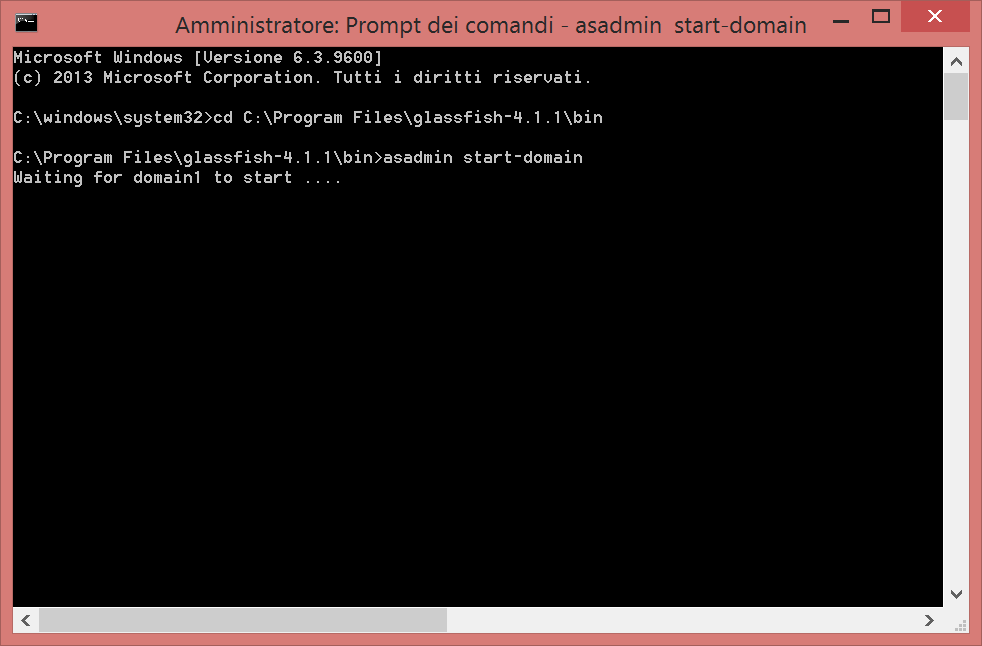
\includegraphics[width=1.1\textwidth]{images/asadminstart}
		\caption{Commands to execute in order to start Glassfish Server}
		\label{asadminstart}
\end{center}
\end{figure}

After the server has started you will be able to access the Admin Console at  \\
\href{url}{https://localhost:4848} and the web server at \\
\href{url}{https://localhost:8080} 
\\(If you need to stop Glassfish server just execute command \textit{asadmin stop-domain}

\subsubsection{Setting up JDK path}
Sometimes an error is displayed if Glassfish does not find the JDK automatically, you can execute the command \\ \textit{asadmin set "server.java-config.java-home=C:\textbackslash Program Files\textbackslash Java\textbackslash jdk1.8.0_121"} \\
Just substitute \textit{C:\textbackslash Program Files\textbackslash Java\textbackslash jdk1.8.0_121} with your path to the JDK you previously downloaded.

\subsubsection{Database configuration}
In order to make it simpler to create the database you can download the already configured Derby database from \\
\href{url}{https://linkdropbox}
\\Unzip it and put it in the folder: \textit{.\textbackslash glassfish\textbackslash databases}\\ in the glassfish installation path (on Windows usually \\
\textit{cd C:\textbackslash Program Files\textbackslash glassfish-4.1.1}
\begin{figure}[H]
\begin{center}
		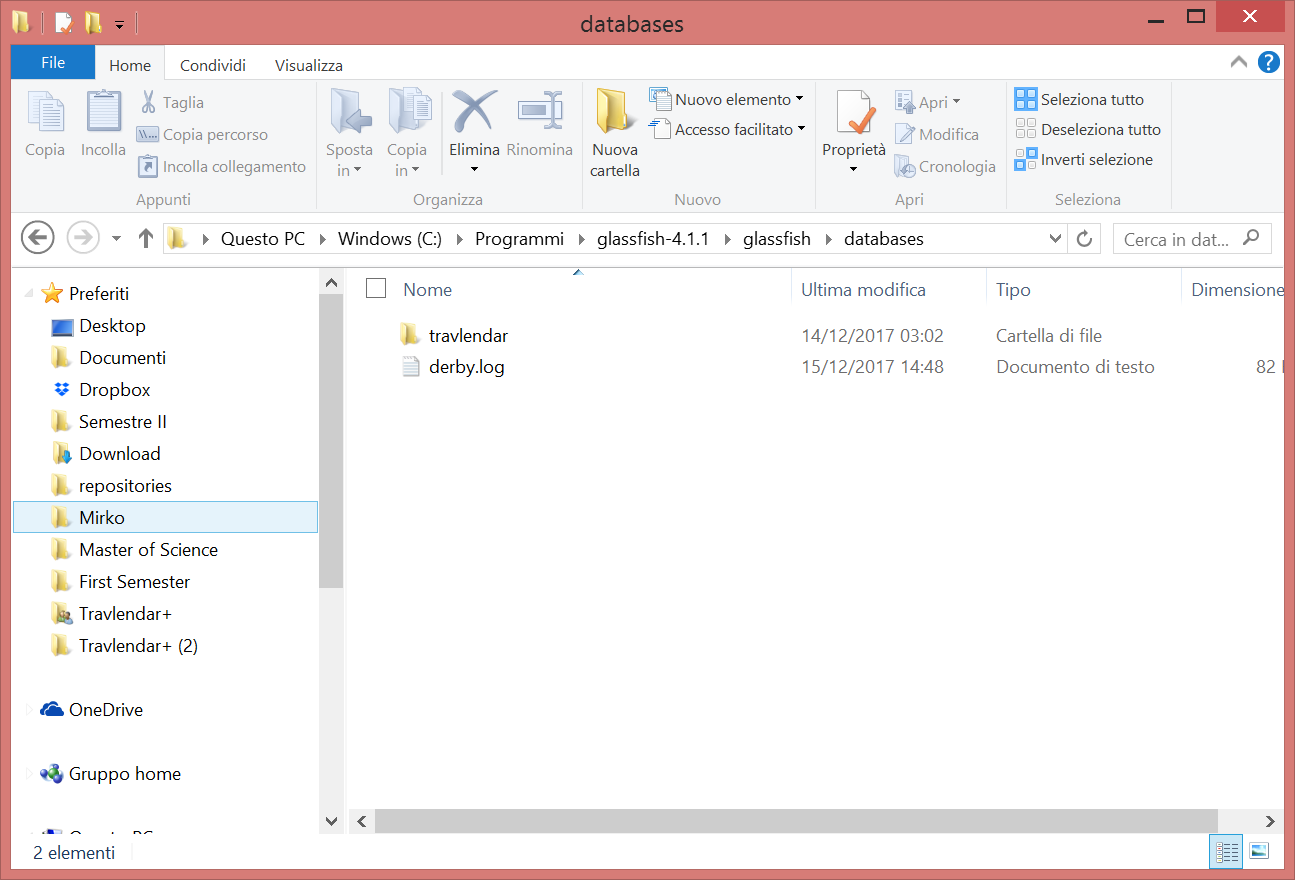
\includegraphics[width=1.1\textwidth]{images/databaselocation}
		\caption{Location in which the database should be stored}
		\label{asadminstart}
\end{center}
\end{figure}


\subsubsection{Starting Apache Derby DBMS}
Execute command \\
\textit{asadmin start-database} \\ in order to start the database. 
\begin{figure}[H]
\begin{center}
		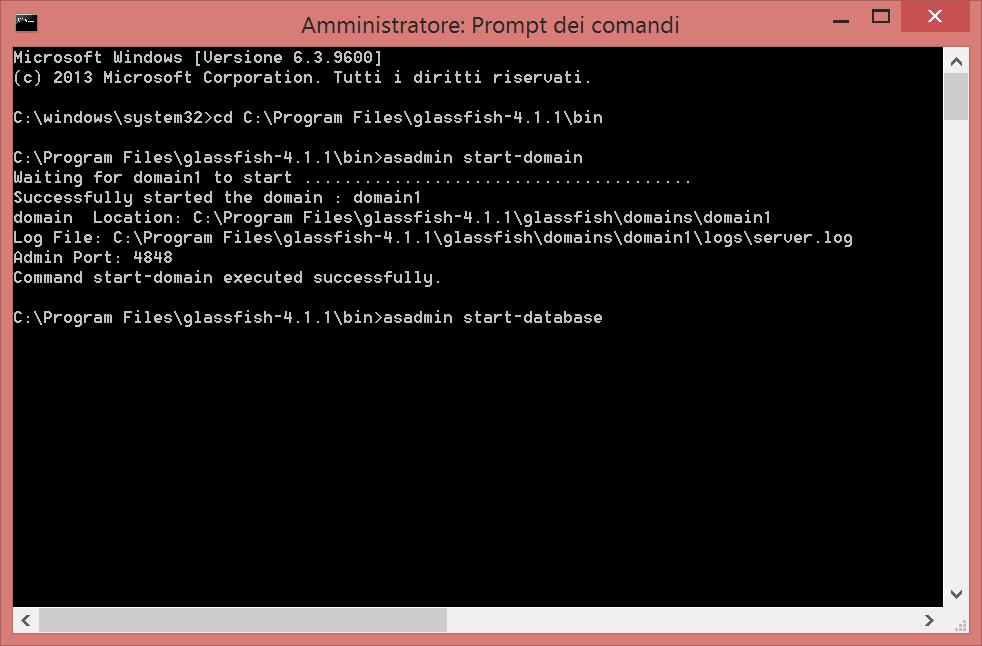
\includegraphics[width=1.1\textwidth]{images/asadmindatabase}
		\caption{Commands to execute in order to start Apache Derby DBMS}
		
\end{center}
\end{figure}
Be sure the port is the default one (1527). \\
If at any moment you want to stop the database just execute command \\
\textit{asadmin stop-database}


\subsection{Application Deployment}
After having configured and set up the environment, download the \texttt{.war} file \texttt{Travlendar.war} at \\
link release in github.
\\You can now follow one of these ways in order to deploy the Application on Glassfish.

\subsubsection{Manual deployment from Admin Console}
After the server has started you will be able to access the Admin Console at  \\
\href{url}{https://localhost:4848}
\\Click on \texttt{Applications} tab on the left. Then click \texttt{Deploy...} button.

\begin{figure}[H]
\begin{center}
		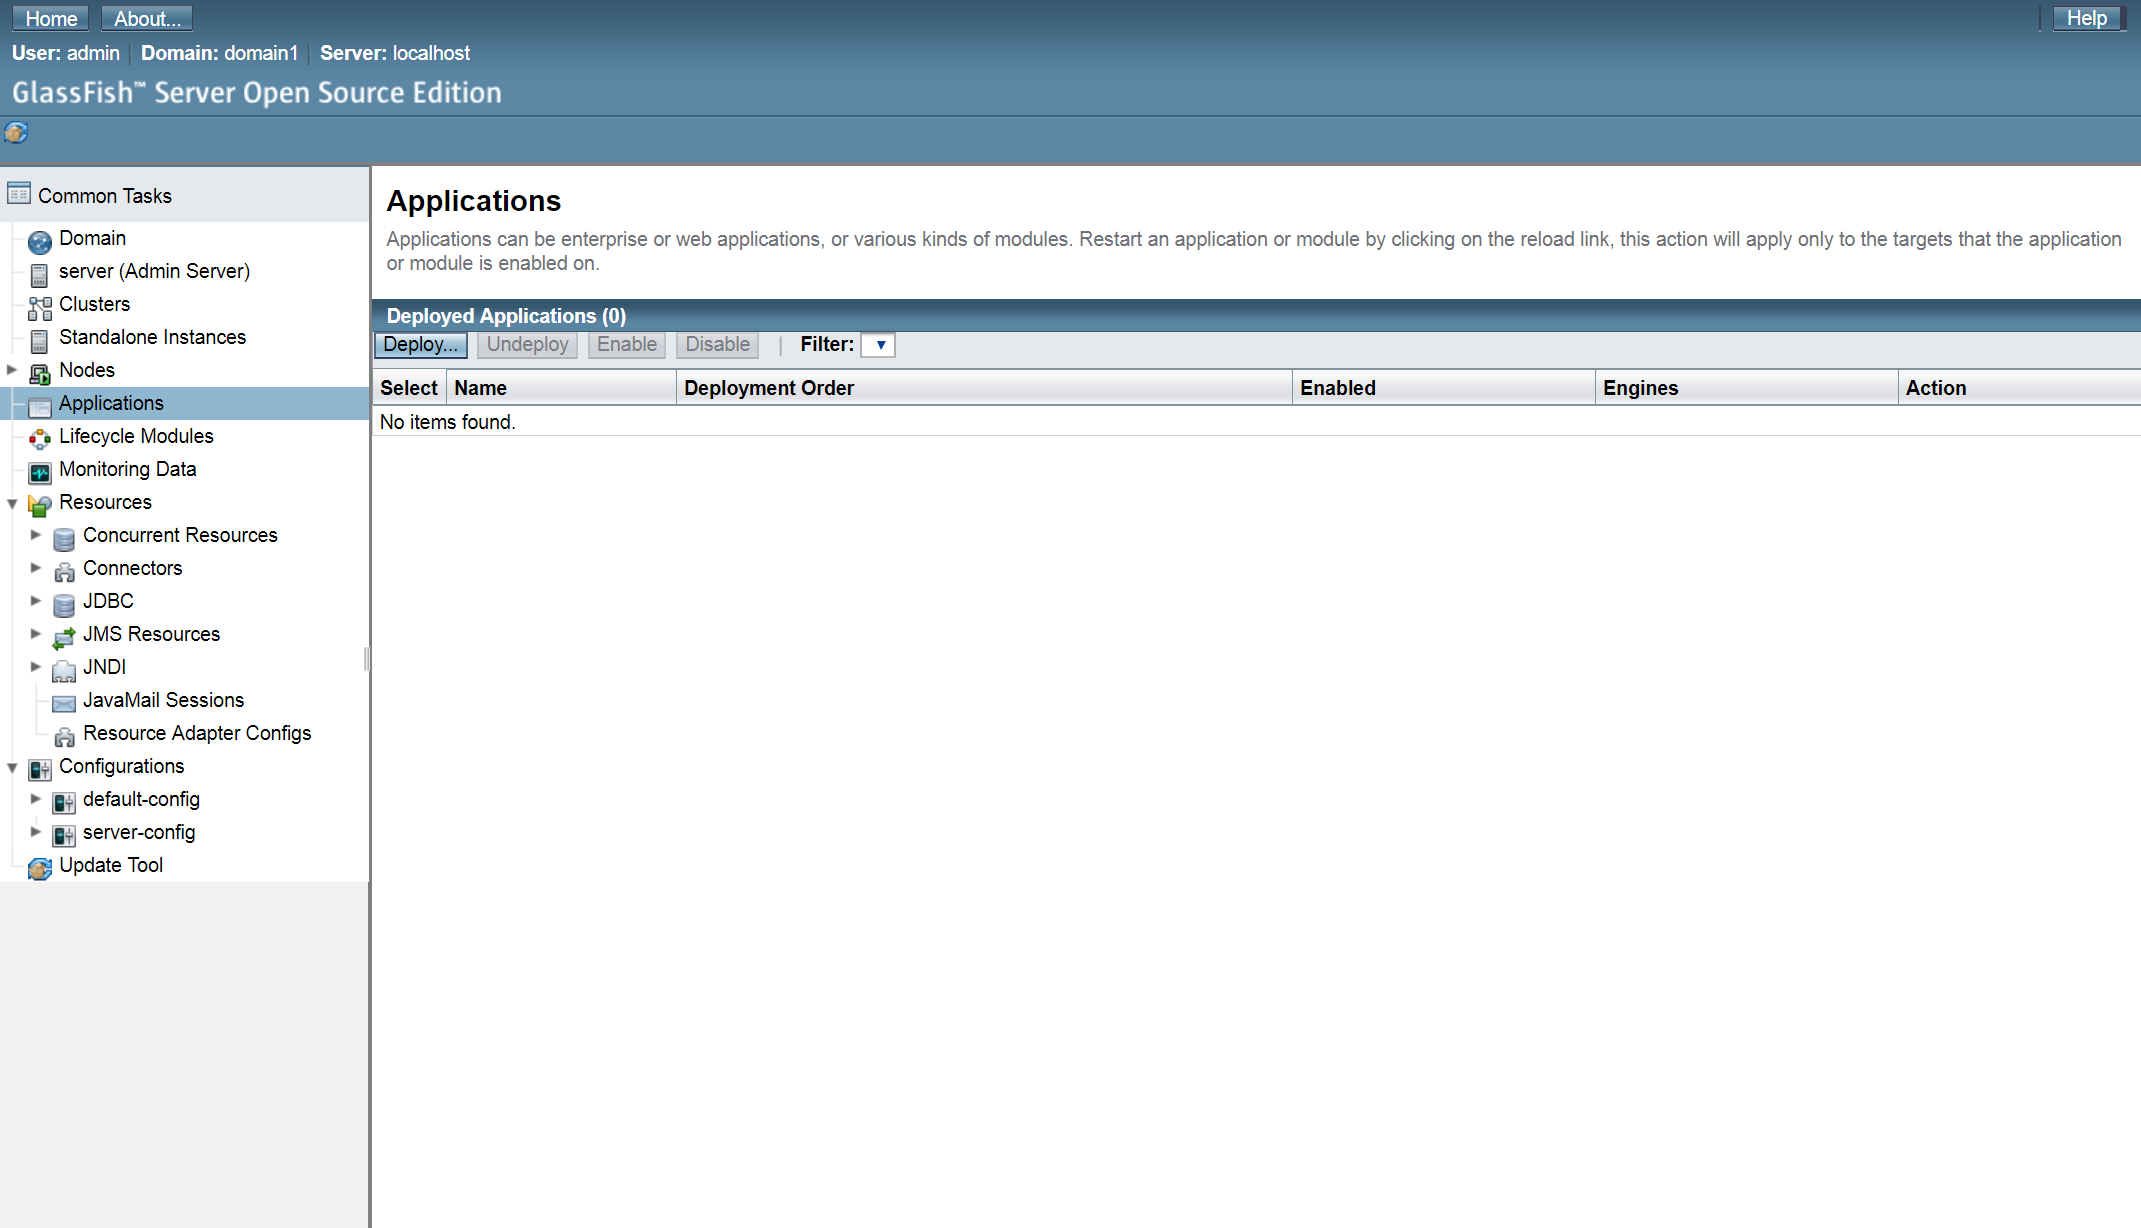
\includegraphics[width=1.1\textwidth]{images/glassfishconsole}
		\caption{Glassfish admin console}
		
\end{center}
\end{figure}

Click on \texttt{Choose file} and select the \texttt{Travlendar.war} release file previously downloaded, then click ok.

\begin{figure}[H]
\begin{center}
		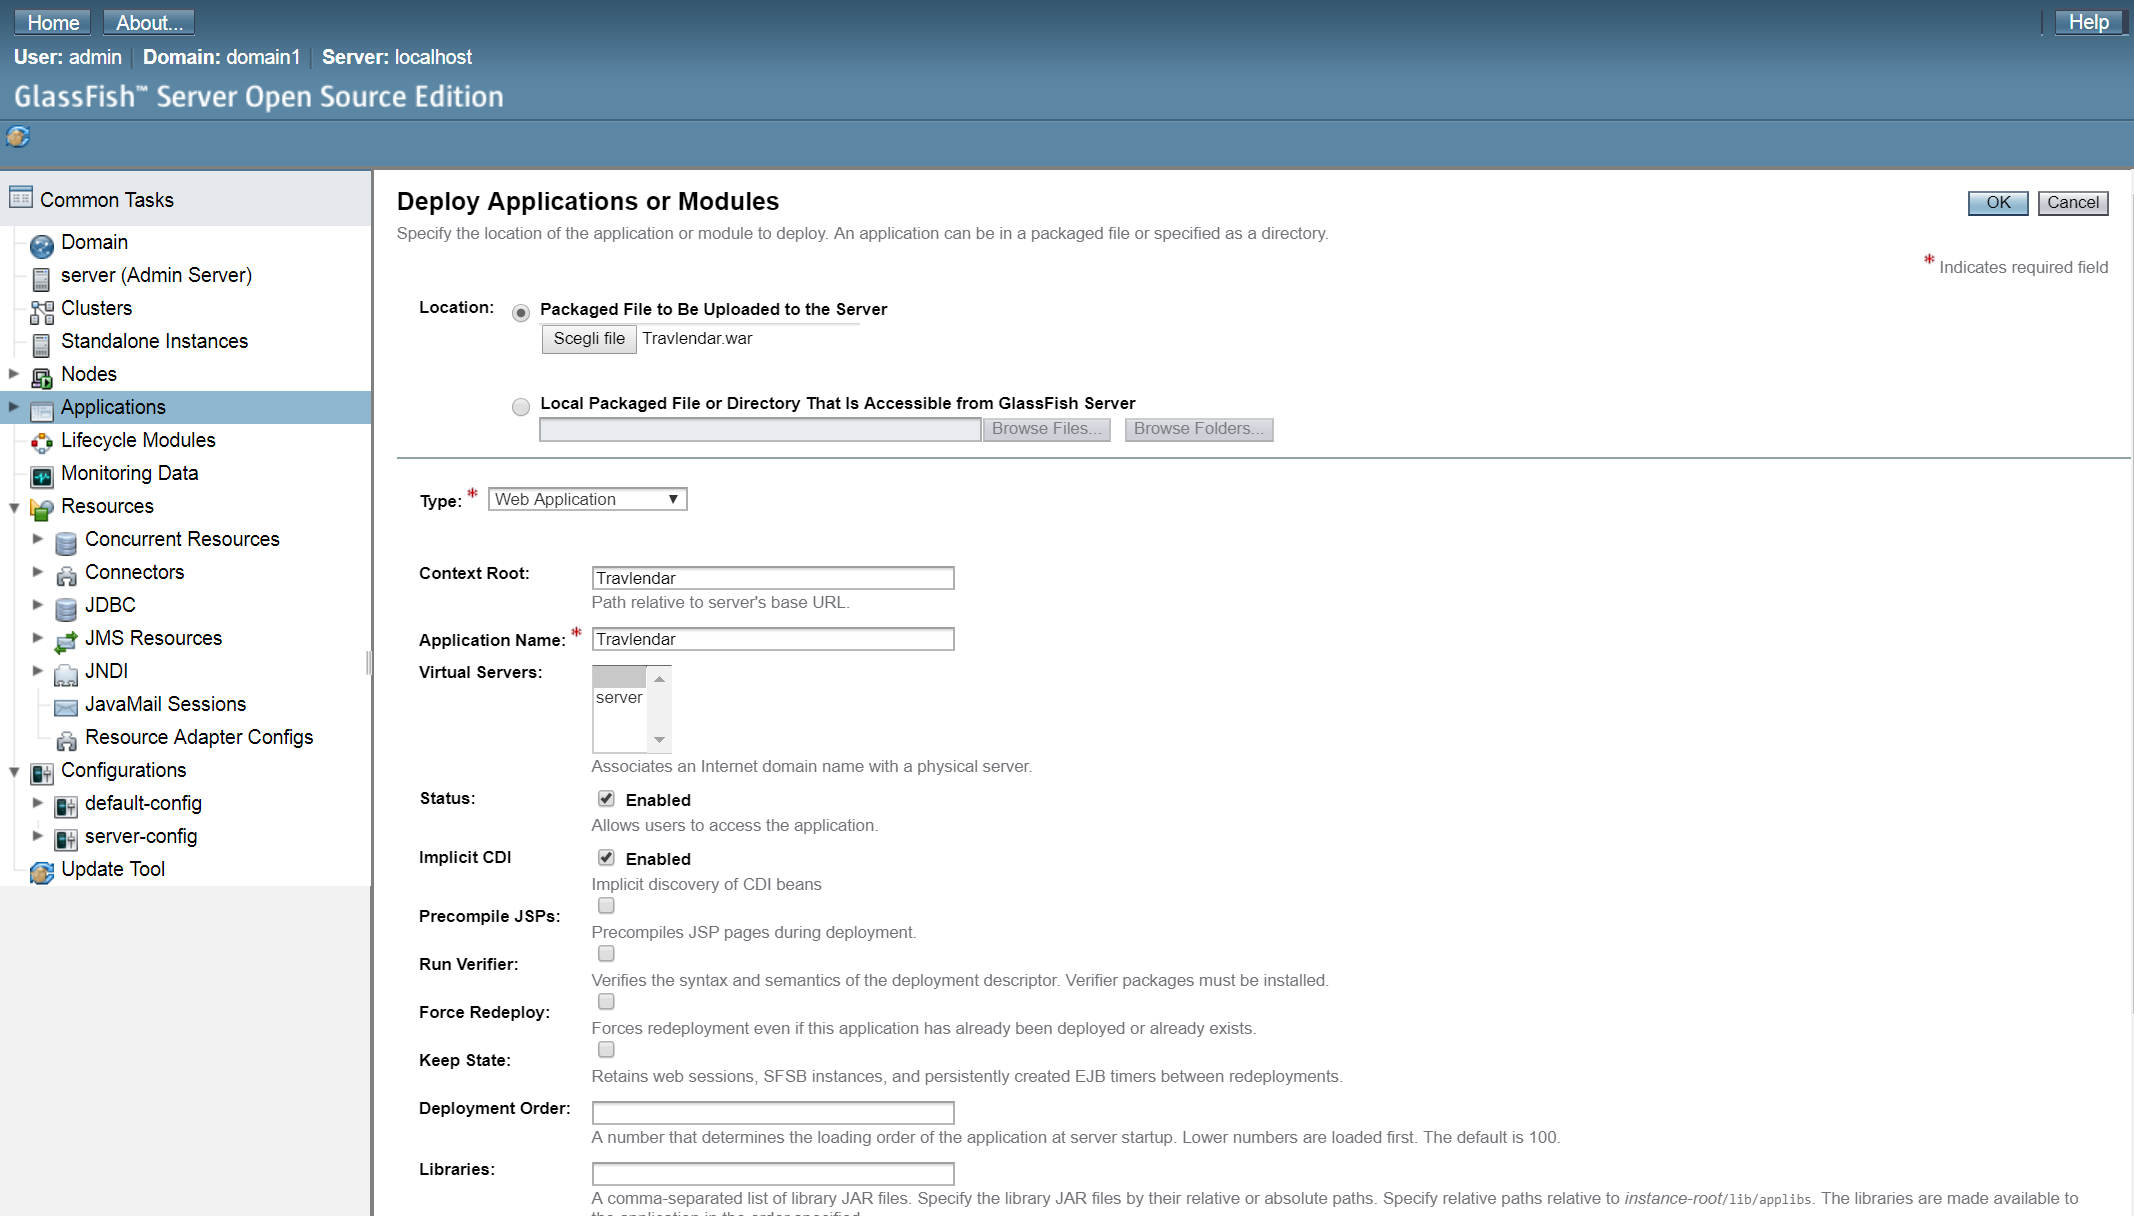
\includegraphics[width=1.1\textwidth]{images/glassfishdeploy2}
		\caption{Glassfish admin console}
		
\end{center}
\end{figure}

If everuthing went fine you should see something similar to this.

\begin{figure}[H]
\begin{center}
		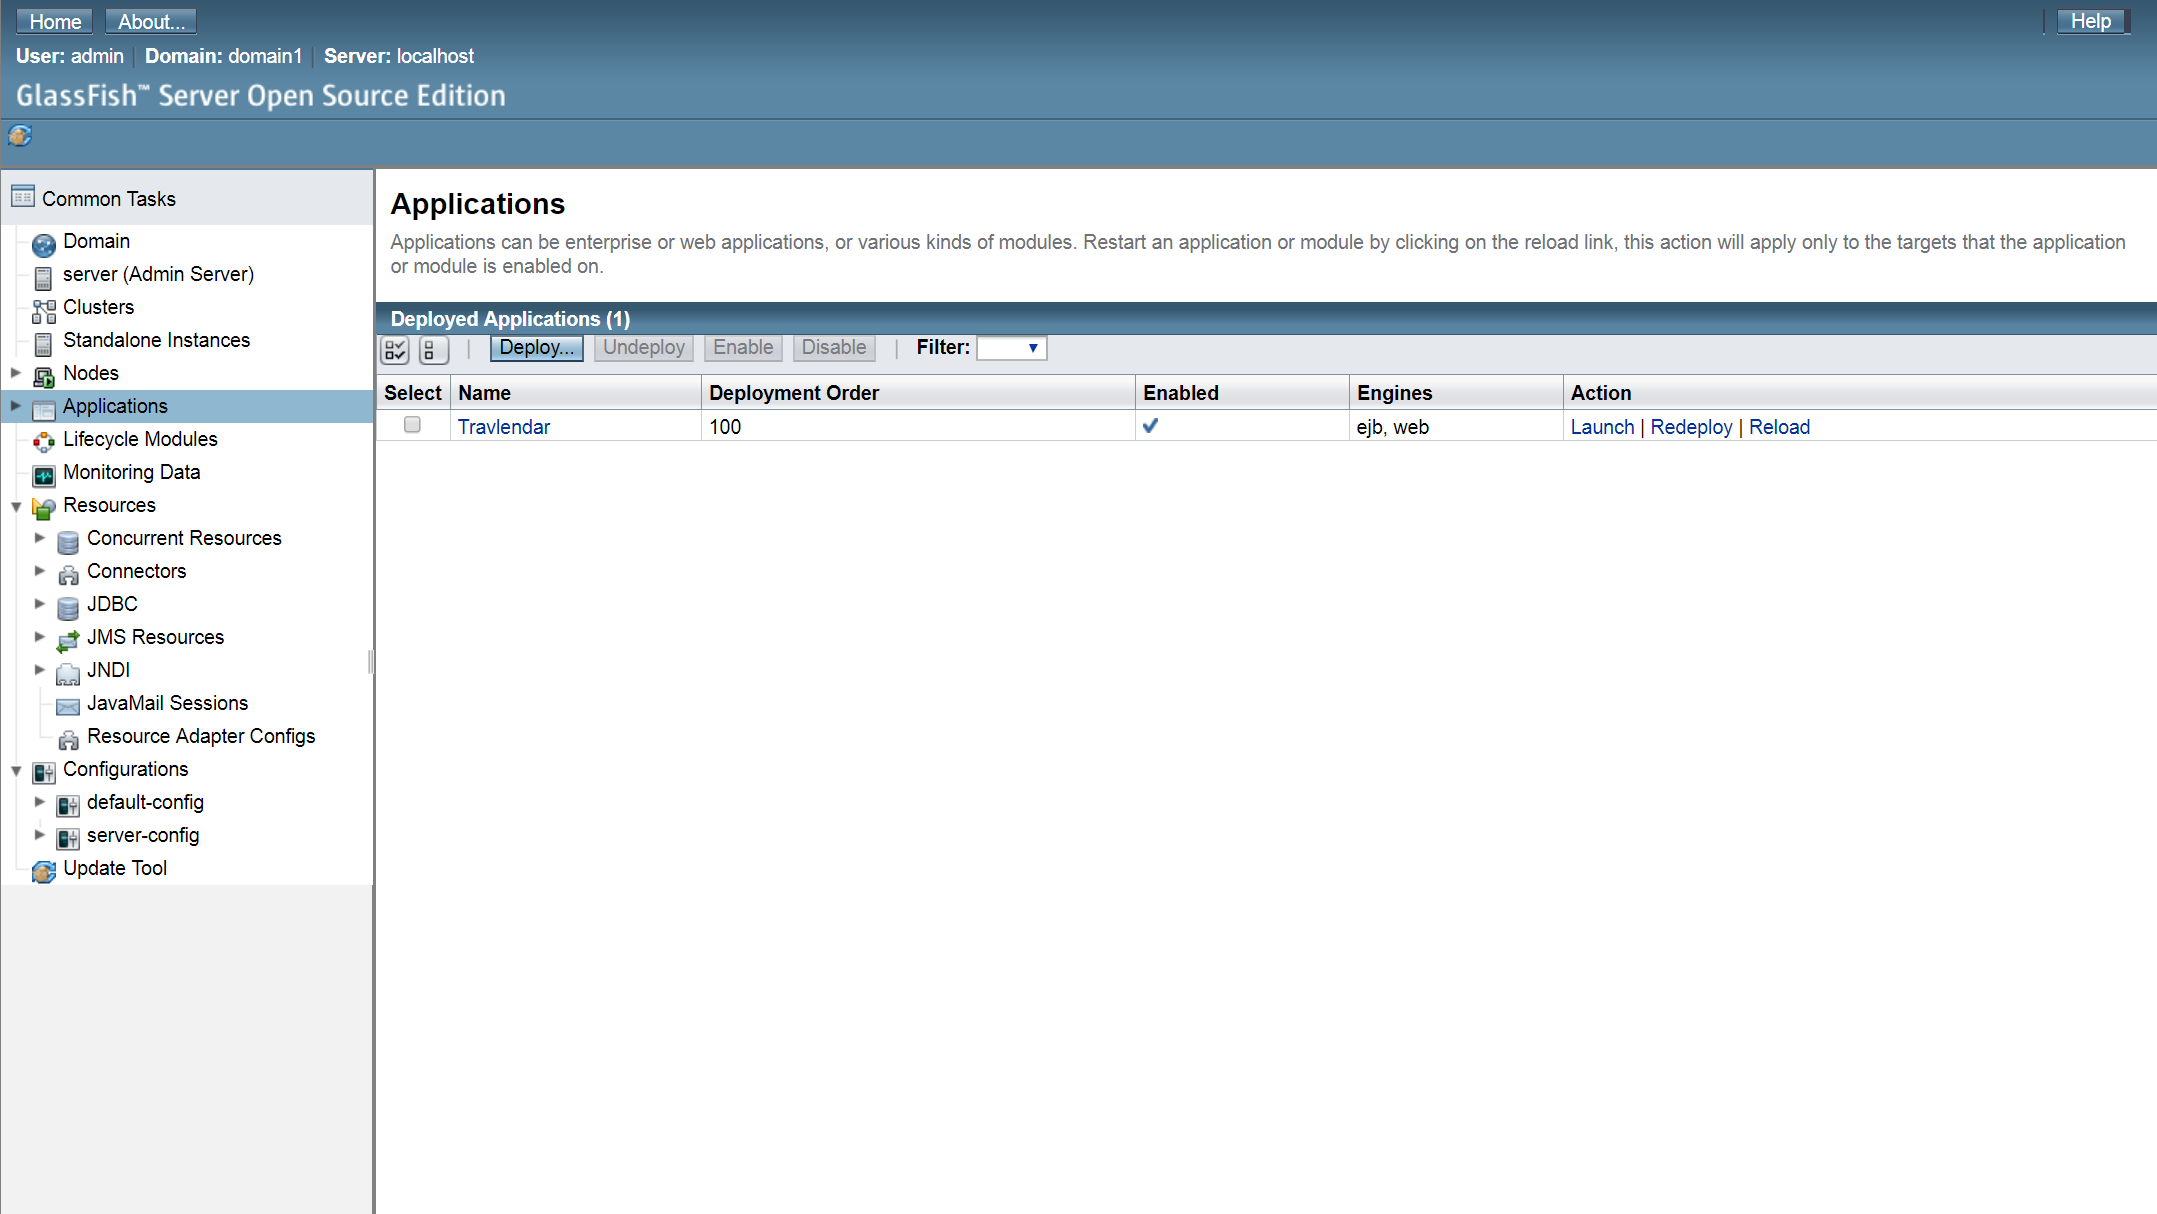
\includegraphics[width=1.1\textwidth]{images/glassfishdeploy}
		\caption{Glassfish admin console}
	
\end{center}
\end{figure}
Just click on \texttt{Launch} to start the application.
\\You can access the application opening the URL: \\
\href{url}{https://localhost:8080/Travlendar}


\subsubsection{Manual deployment from Command Line}
Supposing you already started the server and the database, and you are in the bin folder in the Glassfish installation path, just execute \\ \textit{asadmin deploy C: \textbackslash Users\textbackslash Mirko \textbackslash Desktop\textbackslash Travlendar.war}\\
substituting \textit{C: \textbackslash Users\textbackslash Mirko \textbackslash Desktop\textbackslash} with your path to \texttt{Travlendar.war} release file.

\begin{figure}[H]
\begin{center}
		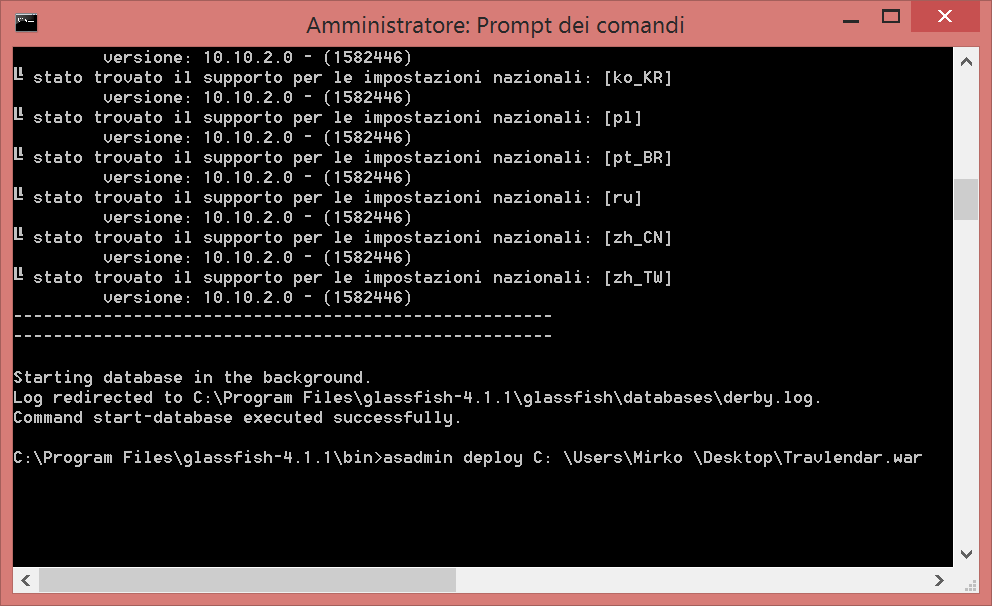
\includegraphics[width=1.1\textwidth]{images/asadmindeploy}
		\caption{Commands to execute in order to Deploy the application on Glassfish Server}
		
\end{center}
\end{figure}

You can now access the application by executing \\
\textit{start http://localhost:8080/Travlendar/} on Windows, \textit{open http://localhost:8080/Travlendar/} on MacOS X, or \textit{xdg-open http://localhost:8080/Travlendar/} on Linux, or simply open the browser and type \textit{localhost:8080/Travlendar} in the URL bar and press Enter.

\subsubsection{Autodeployment}
Just put the \texttt{Travlendar.war} file in \textit{<GlassFish-Installation-Path>/domains/domain1/autodeploy} and restart the server.

\subsection{Running the app}
Once the deployment is finished you can access the Application at \textit{localhost:8080/Travlendar}
on a browser in your local machine, at \textit{192.168.1.3:8080/Travlendar} on a device connected to the same LAN (just replace \textit{192.168.1.3} with the private IP address of the machine the server is running on. 
\\You can even access the application from a remote device, you just need to open the port 8080 of the router of your LAN by creating a virtual server and NATting the external access onto the private IP address of the machine your server is running on (private IP should be configured as static). Then you can access from wherever you want just by going to \textit{xx.xx.xx.xx:8080/Travlendar}, replace xx.xx.xx.xx with the public IP address of your router.

\begin{figure} 
\begin{center}

\makebox[\textwidth]{%
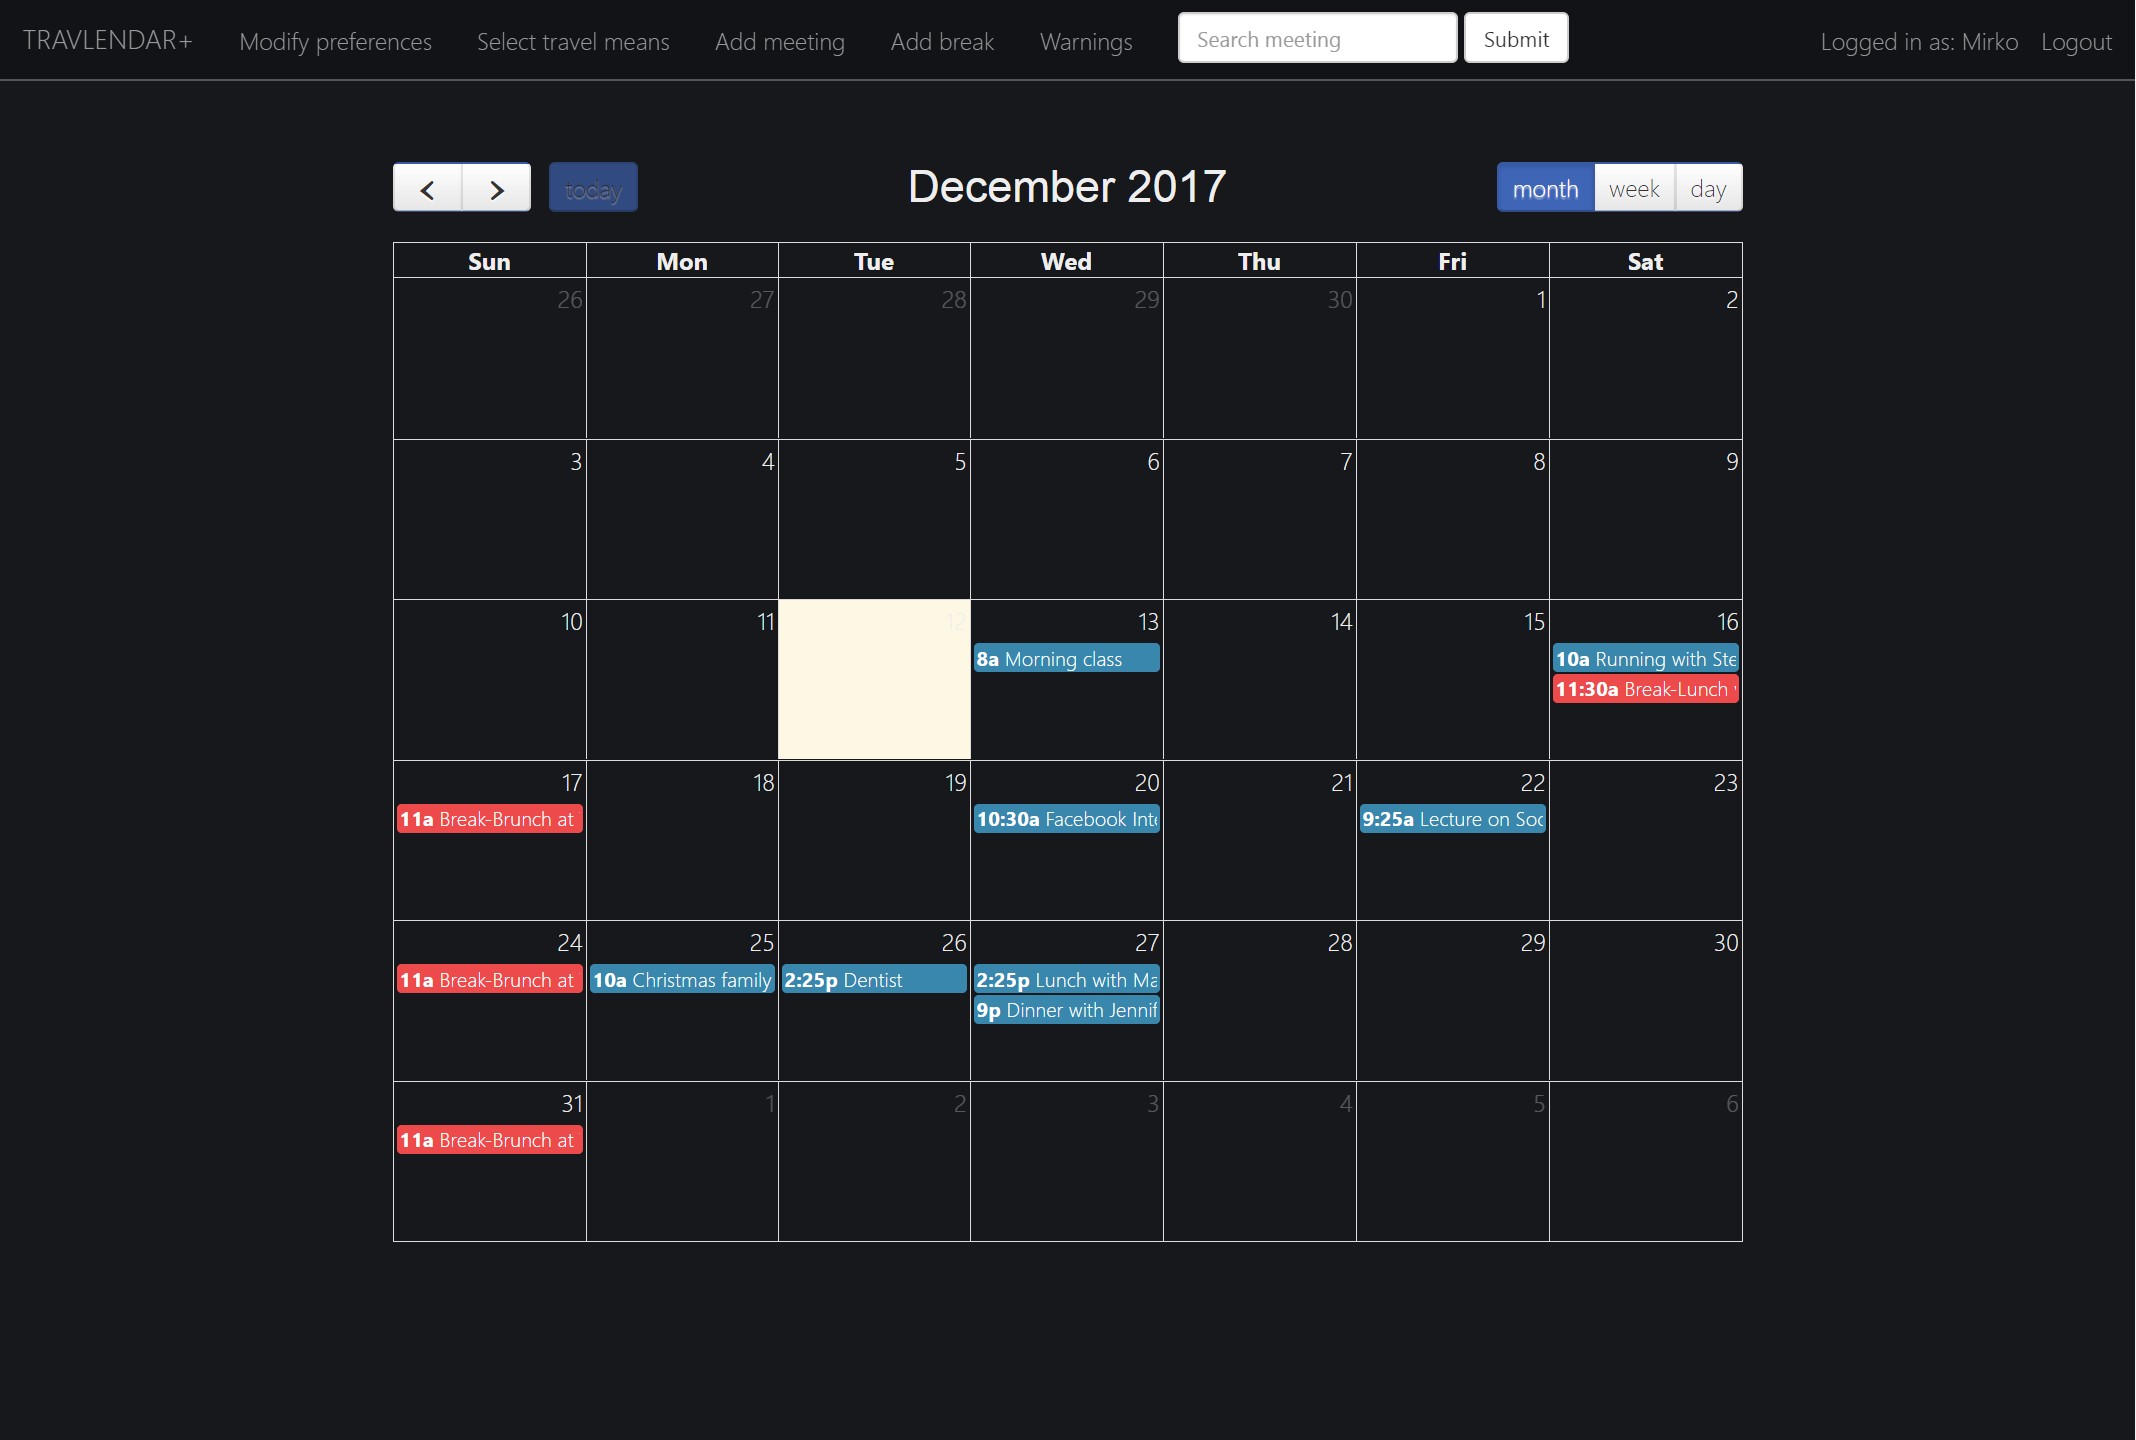
\includegraphics[width=1.5\linewidth]{images/homepage} 
}
\caption{Travlendar Homepage} 
\label{fig:travlendarhomepage} 


\end{center}
\end{figure} 

\clearpage
\subsection{Possible issues and solutions}
If you encounter any problem in the deployment regarding a database connectivity problem you could download Netbeans IDE (which includes Glassfish and Derby installation) and replace the Environment setup steps by creating a database with databasename = travlendar, name = mirko, password = mirko.
Start glassfish server from there and then pass to the deployment phase as explained in these instructions.
\\If also this does not let you deploy the app as last chance you could clone the travlendar repository, import it as a project in netbeans build and clean the project, and run it.




\clearpage
\section{Appendix}

\subsection{Used software}
\begin{center}
	
	\-\\
	\begin{tabular}{*{2}{c}}
		\toprule
		Task & Software \\
		\midrule
		Edit and compile \LaTeX\ code & TeXmaker, TeXstudio\\
		Development IDE & Netbeans\\
		Application server & Glassfish 4.1.1\\
		DBMS & Java DB (Derby)\\
		\bottomrule
	\end{tabular}
\end{center}

\subsection{Effort spent}
\begin{itemize}

\item Matteo Marziali working hours:  $\approxeq$ 100 hours

\item Mirko Mantovani working hours:  $\approxeq$ 100 hours



\end{itemize}



\end{document}
